\documentclass[conference,a4paper]{IEEEtran}

\usepackage[T1]{fontenc}
\usepackage[utf8]{inputenc}
\usepackage{microtype}
\usepackage{booktabs}
\usepackage{array}
\usepackage{graphicx}
\usepackage{xcolor}
\usepackage{amsmath}
\usepackage{cite}
\usepackage{hyperref}
\usepackage{tikz}
\usetikzlibrary{arrows.meta,positioning,fit}
\usepackage{pgfplots}
\pgfplotsset{compat=1.18,compat/show suggested version=false}

\hypersetup{colorlinks=true,linkcolor=black,citecolor=black,urlcolor=blue,pdfauthor={}}
\setlength{\emergencystretch}{1em}
\renewcommand{\arraystretch}{1.08}

\title{Extraction of Reference Components\\
from Low-Resource Documents}
\author{\IEEEauthorblockN{Anonymous Authors}}

\begin{document}
\maketitle

\begin{abstract}
This paper addresses fine-grained extraction of reference components from Hebrew-Aramaic Jewish Responsa dating approximately from the eighteenth through twenty-first centuries. The task is formulated as named-entity recognition over eight component types, including authors, books, sections, chapters, sub-chapters, and their lexical prefixes. The initial corpus contains 150 manually annotated sentences (3,012 tokens, including 480 entity tokens). We compare DictaBERT and BEREL 3.0 under random and label-aware greedy sentence splits. The evaluated architectures comprise direct NER, a typed three-step cascade, local BIO repair, confidence fusion, and a linear SVM router that resolves disagreements between the direct and cascaded outputs. Performance is measured by strict entity-level micro-F1 over 20 seed-indexed runs. DictaBERT with label-aware splitting and SVM fusion obtains the highest mean F1 of 0.781. BEREL 3.0 consistently achieves higher direct-NER F1, whereas DictaBERT yields the highest fused F1. Relative to the encoder-matched Random-split Direct-NER baseline, all four SVM-fusion conditions are significant under paired Wilcoxon tests with Holm correction at $\alpha=0.01$. The results demonstrate the importance of split composition and complementary prediction structures in extremely low-resource historical-language NER.
\end{abstract}

\begin{IEEEkeywords}
named-entity recognition, Hebrew, Aramaic, Responsa, low-resource NLP, citation extraction
\end{IEEEkeywords}

\section{Introduction}

Jewish Responsa are legal and scholarly texts whose arguments frequently cite earlier authorities, books, tractates, chapters, sections, and smaller textual units. Structured extraction of these components supports retrieval, bibliographic normalization, and computational analysis of relationships among cited sources.

The collection examined in this study spans approximately the eighteenth through twenty-first centuries.

Responsa citations lack a standardized bibliographic syntax. They may be abbreviated, incomplete, or embedded in extended argumentation, and they combine historical Hebrew, Aramaic, spelling variation, and domain-specific terminology. Earlier work on biblical-quotation identification and Hebrew-Aramaic abbreviation disambiguation demonstrates the need for domain-specific handling of partial references and shortened forms \cite{hacohen2010,hacohen2010haads}. Hebrew cliticization further complicates token boundaries and lexical interpretation \cite{mordecai2005hebrew,itai2008,tsarfaty2019hebrewnlp}. The resulting task differs substantially from conventional news-domain NER.

We report a controlled initial experiment on 150 labeled sentences using an approximately 70/30 train--evaluation division. The comparison is restricted to DictaBERT, BEREL 3.0, direct NER, a typed three-step cascade, local consistency repair, and two fusion strategies. Random and label-aware sentence splitting are evaluated.

The contributions are:

\begin{itemize}
  \item a fine-grained NER formulation covering eight Responsa reference components;
  \item a controlled comparison of Modern-Hebrew and rabbinic-Hebrew encoders under random and label-aware sentence splits;
  \item a typed cascade that decomposes entity detection, BIO position, and component-type prediction; and
  \item paired significance testing of direct and fused outputs.
\end{itemize}

The proposed design addresses low-resource imbalance at three levels. The label-aware split controls which rare labels are available during training and evaluation; the cascade separates the dominant entity-versus-\texttt{O} decision from boundary and type learning; and the fusion stage learns when the direct and decomposed views are complementary. The contribution is therefore primarily in data allocation and prediction-pipeline design rather than in introducing another pretrained encoder.

\section{Related Work}

Sequence labeling progressed from conditional random fields \cite{lafferty2001crf} and neural BiLSTM--CRF architectures \cite{ma2016bilstmcrf} to contextual transformer encoders \cite{devlin2018bert}; Li et al. \cite{li2022ner} survey this broader development in NER. DictaBERT provides pretrained representations for Modern Hebrew \cite{shmidman2023dictabert}, whereas BEREL was trained on rabbinic language and is consequently closer to the domain examined here \cite{shmidman2022berel}.

Hebrew NER is affected by rich morphology and limited annotated resources \cite{mordecai2005hebrew,itai2008,tsarfaty2019hebrewnlp}. Responsa introduce additional ambiguity because authors, works, sections, and locators often occur in abbreviated or lexically overlapping forms.

Nguyen et al. \cite{nguyen2023auc} decompose low-resource NER into entity detection and boundary prediction. We extend this formulation with an explicit component-type head, enabling reconstruction of complete typed BIO labels rather than untyped entity spans.

Because several labels are rare, partition composition is a central experimental factor. Class-imbalance studies emphasize the risk of majority-class dominance \cite{japkowicz2002}, while evaluation research shows that data allocation can materially affect estimates obtained from small samples \cite{kohavi1995}. We therefore compare random allocation with corpus-specific label-aware greedy allocation.

\section{Dataset and Task}

\subsection{Corpus}

The corpus contains 150 manually annotated Responsa sentences dating approximately from the eighteenth through twenty-first centuries. The annotated sample contains 3,012 tokens: 480 entity tokens and 2,532 \texttt{O} tokens. The annotations comprise 399 entity spans, and entity tokens account for 15.9\% of the corpus.

Table~\ref{tab:labels} reports the eight component types. Their frequencies are strongly skewed: author tokens are dominant, whereas section-prefix tokens are scarce. This imbalance makes the evaluation sensitive to sentence allocation.

\begin{table}[!t]
\centering
\caption{Entity-token counts in the 150-sentence corpus, sorted by frequency. Prefix labels identify words that introduce a component.}
\label{tab:labels}
\small
\begin{tabular}{@{}llr@{}}
\toprule
Code & Component & Token count \\
\midrule
\texttt{AUT} & Author & 171 \\
\texttt{BOK} & Book & 91 \\
\texttt{CHP} & Chapter & 71 \\
\texttt{SEC} & Section & 41 \\
\texttt{pCHP} & Chapter prefix & 41 \\
\texttt{SCHP} & Sub-chapter & 28 \\
\texttt{pSCHP} & Sub-chapter prefix & 27 \\
\texttt{pSEC} & Section prefix & 10 \\
\midrule
 & Total & 480 \\
\bottomrule
\end{tabular}
\end{table}

\subsection{Annotation and task formulation}

For a token sequence $x=(x_1,\ldots,x_n)$, the model predicts $y=(y_1,\ldots,y_n)$ from
\begin{equation}
\mathcal Y=\{\texttt{O}\}\cup
\{\texttt{B-}t,\texttt{I-}t:t\in\mathcal T\},
\end{equation}
where $\mathcal T$ contains the eight component types in Table~\ref{tab:labels}; hence $|\mathcal Y|=17$. For example, the transliterated citation ``Rambam, perek tet-zayin, Hilkhot Issurei Biah'' contains an author, a chapter prefix, a chapter, and a section. All partitions are performed at sentence level to prevent cross-partition leakage.

The principal ambiguities arise from class imbalance, abbreviation, and contextual overlap between bibliographic roles. In particular, work titles may occur in author-like syntactic contexts, making book--author distinctions dependent on both lexical identity and surrounding context.

\section{Methods}

\subsection{Encoders}

We compare DictaBERT, pretrained primarily for Modern Hebrew, with BEREL 3.0, whose rabbinic-language pretraining is more closely matched to the target domain. Each encoder is fine-tuned independently for the direct and cascaded prediction sources under identical task definitions, partitions, and evaluation criteria.

\subsection{Direct NER}

Let $h_i$ denote the contextual representation of token $i$. The direct model predicts the complete typed BIO label using a linear classification head:

\begin{equation}
  \mathbf{s}_i=W h_i+\mathbf{b},\qquad
  \hat y_i=\arg\max_{y\in\mathcal Y}s_{i,y}.
\end{equation}

Training minimizes token-level cross-entropy with padding positions masked. The model also exports the selected-label posterior and the top-two posterior margin for downstream fusion.

\subsection{Typed three-step cascade}

The cascade applies three classification heads to the shared contextual representation: entity membership $e_i\in\{0,1\}$, BIO position $b_i\in\{\texttt{B},\texttt{I}\}$, and component type $t_i\in\mathcal T$. Their predictions are reconstructed as

\begin{equation}
\begin{aligned}
z_i^{e}&=W_eh_i+b_e, &
z_i^{b}&=W_bh_i+b_b,\\
\mathbf z_i^{t}&=W_th_i+\mathbf b_t.
\end{aligned}
\end{equation}

The entity and boundary heads are binary, while the type head applies a softmax over the eight component types. For a gold \texttt{O} token, only the entity target is defined; its boundary and type targets are masked. A gold entity token supplies supervision to all three heads. The final typed label is reconstructed as

\begin{equation}
\hat y_i=
\begin{cases}
\texttt{O}, & \hat e_i=0,\\
\hat b_i\texttt{-}\hat t_i, & \hat e_i=1.
\end{cases}
\end{equation}

The entity loss is evaluated on all non-padding tokens, whereas the boundary and type losses are evaluated only on gold entity tokens. This conditional masking prevents the majority \texttt{O} class from dominating decisions that are meaningful only inside entities. The training objective is

\begin{equation}
\mathcal L=\mathcal L_{entity}
+\lambda_{bio}\mathcal L_{boundary}+\lambda_{type}\mathcal L_{type}.
\end{equation}

We set default $\lambda_{bio}=10$ and $\lambda_{type}=5$, and select coefficients from a coarse validation grid $\lambda_{bio},\lambda_{type}\in\{1,5,10\}$ (nine configurations) on the same 70/30 sentence split used for threshold tuning. The chosen pair maximizes validation pipeline span F1 in predicted mode after the internal threshold sweep; the test set is not used for this search (see \texttt{experiment\_04\_loss\_weight\_grid.py}). Boundary and type terms apply to fewer gold entity tokens than the entity term; the weights balance their gradient contribution through the shared encoder. Unlike a fixed $0.5$ decision rule, the implementation calibrates separate entity and boundary thresholds over
$\{0.10,0.15,\ldots,0.90\}$. The selected pair maximizes the combined entity-detection and boundary F1 objectives:

\begin{equation}
(\tau_e^*,\tau_b^*)=
\arg\max_{\tau_e,\tau_b}
\left(F1_e(\tau_e)+F1_b(\tau_b)\right).
\end{equation}

This decomposition isolates three sources of error---entity presence, span position, and semantic type---while still producing the same 17-label output space as direct NER. The architecture extends Nguyen et al. \cite{nguyen2023auc} by adding explicit typed prediction.

\subsection{Consistency repair}

The repair variant applies deterministic local constraints to the reconstructed sequence. An \texttt{I} tag at sentence onset, after \texttt{O}, or after an incompatible type is converted to the corresponding \texttt{B} tag. No additional parameters are trained.

\subsection{Fusion}

\textbf{Confidence fusion} combines the direct and cascaded predictions without retraining either source. Let $\hat y_i^d$ and $\hat y_i^c$ be their predicted labels for token $i$, and let $p_i^d$ and $p_i^c$ be the corresponding confidence scores. The direct confidence is the posterior probability assigned to its selected 17-class BIO label. For the cascade, let $p_i^e$ be the probability that the token is an entity and let $p_i^b$ be the probability assigned to its selected \texttt{B}/\texttt{I} position. Its confidence is

\begin{equation}
p_i^c=
\begin{cases}
1-p_i^e, & \hat y_i^c=\texttt{O},\\
p_i^e p_i^b, & \hat y_i^c\ne\texttt{O}.
\end{cases}
\end{equation}

Thus, an entity prediction receives high cascade confidence only when both entity membership and BIO position are confident. The fused label is

\begin{equation}
\hat y_i^{f}=\begin{cases}
\hat y_i^d, & \hat y_i^d=\hat y_i^c,\\
\hat y_i^d, & \hat y_i^d\ne\hat y_i^c \text{ and } p_i^d\ge p_i^c,\\
\hat y_i^c, & \text{otherwise.}
\end{cases}
\end{equation}

Agreements are therefore retained directly. For a disagreement, the source with higher confidence is selected; if the confidence scores are equal, the direct-NER label is selected deterministically.

\textbf{SVM fusion} trains a linear router only on tokens for which the direct and cascaded labels disagree. A router target is retained when one source matches the gold token label; disagreements for which neither source is correct are uninformative for source selection and are discarded. Let $m_i^d$ and $m_i^c$ denote the probability margins of the direct and cascaded sources, respectively, where each margin is the difference between the highest and second-highest relevant prediction probabilities. The numeric feature vector is

\begin{equation}
\begin{aligned}
\phi_i^{num}=\big[&p_i^d,\ p_i^c,\ m_i^d,\ m_i^c,\\
&p_i^d-p_i^c,\ \lvert p_i^d-p_i^c\rvert,\
\max(p_i^d,p_i^c)\big].
\end{aligned}
\end{equation}

The features therefore include the regular/direct-NER probability, the cascaded probability, both probability margins, the signed probability difference, the absolute probability difference, and the maximum of the two probabilities. Predicted BIO positions and component types from both sources are additionally one-hot encoded, while the numeric features are standardized. A class-balanced linear SVM with $C=1$ learns

\begin{equation}
f(\phi_i)=w^T\phi_i+b,
\end{equation}

whose sign selects the direct or cascaded label. Agreement tokens bypass the router. When the disagreement sample is insufficient for training, confidence fusion is used as a fallback.

\subsection{Sentence splits}

All conditions use an approximately 70/30 sentence-level division. Let $c_A(\ell)$ denote the number of tokens with non-\texttt{O} label $\ell$ in sentence subset $A$, and let the target training count be $q_\ell=0.7c_D(\ell)$.

\begin{itemize}
  \item \textbf{Random}: seeded random sentence assignment.
  \item \textbf{Label-aware greedy}: the training partition is constructed one sentence at a time. At each step, candidate sentences are scored by their effect on
  \begin{equation}
  J(A)=\sum_{\ell\ne\texttt{O}}
  \left(c_A(\ell)-q_\ell\right)^2,
  \end{equation}
  and the sentence that best reduces the label-count mismatch is selected. Rare labels with a large remaining deficit therefore receive priority while the training-size constraint is maintained.
\end{itemize}

\begin{figure*}[!t]
\centering
\resizebox{0.94\textwidth}{!}{%
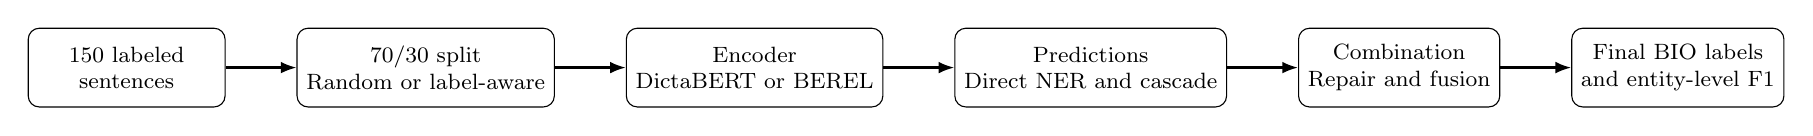
\begin{tikzpicture}[
  node distance=9mm,
  box/.style={draw,rounded corners,align=center,minimum height=10mm,minimum width=25mm,font=\footnotesize,fill=white},
  arrow/.style={-{Latex[length=2mm]},thick}
]
\node[box] (data) {150 labeled\\sentences};
\node[box,right=of data] (split) {70/30 split\\Random or label-aware};
\node[box,right=of split] (encoder) {Encoder\\DictaBERT or BEREL};
\node[box,right=of encoder] (models) {Predictions\\Direct NER and cascade};
\node[box,right=of models] (fusion) {Combination\\Repair and fusion};
\node[box,right=of fusion] (output) {Final BIO labels\\and entity-level F1};

\draw[arrow] (data) -- (split);
\draw[arrow] (split) -- (encoder);
\draw[arrow] (encoder) -- (models);
\draw[arrow] (models) -- (fusion);
\draw[arrow] (fusion) -- (output);
\end{tikzpicture}
}
\caption{Basic experimental flow from the annotated corpus to the final predictions and F1 evaluation.}
\label{fig:process}
\end{figure*}

\section{Experimental Setup}

Each split assigns approximately 105 sentences to training and 45 to evaluation. The experiment contains 20 seed-indexed records per encoder, method, and split condition (seeds 42--61). Comparisons are aligned by seed, and F1 results are reported as mean and sample standard deviation. Deterministic partitioning conditions yield identical records where applicable and consequently have zero standard deviation.

The primary measure is strict entity-level micro-F1 under exact span and component-type matching. Token accuracy is not used as the principal criterion because 84.1\% of corpus tokens carry the majority \texttt{O} label, which can make accuracy misleading in imbalanced classification \cite{sokolova2009measures}. Thus, boundary and type errors both invalidate an entity prediction.

The five evaluated outputs are direct NER, the raw typed cascade, the repaired cascade, confidence fusion, and SVM fusion. Repair and fusion operate on existing predictions and do not require an additional transformer. Figure~\ref{fig:process} summarizes the experimental dependencies.

For each encoder, Random-split Direct NER is the statistical baseline. Each SVM-fusion condition is paired with this baseline by seed, producing four planned comparisons: two splits for each of the two encoders. A second family of four tests compares DictaBERT and BEREL 3.0 under matched seeds for Direct NER and SVM fusion across the two splits. We apply two-sided Wilcoxon signed-rank tests; Holm correction is applied separately within each four-test family, and significance is assessed at $\alpha=0.01$. For cross-split comparisons, seed alignment identifies corresponding runs but does not imply that the evaluation sentences are identical.

\section{Results}

Table~\ref{tab:results} presents the complete F1 comparison. DictaBERT with label-aware splitting and SVM fusion achieves the highest mean F1 of 0.781, giving an F1 gain of 0.124 over the corresponding direct model and an F1 gain of 0.119 over DictaBERT SVM fusion under random splitting.

\begin{table}[!t]
\centering
\caption{Strict entity-level F1 on the 150-sentence experiment (mean $\pm$ standard deviation over the exported seed-indexed records). Bold marks the best result in each encoder--split column; Random Direct NER is the statistical baseline.}
\label{tab:results}
\scriptsize
\begin{tabular}{@{}lcc@{}}
\toprule
Method & Random & Label-aware \\
\midrule
\multicolumn{3}{@{}l}{\textbf{BEREL 3.0}}\\
Direct NER & $0.623\pm0.021$ & $0.683\pm0.000$ \\
Three-step cascade & $0.333\pm0.090$ & $0.301\pm0.089$ \\
Cascade + repair & $0.333\pm0.091$ & $0.302\pm0.091$ \\
Confidence fusion & $0.492\pm0.083$ & $0.523\pm0.052$ \\
SVM fusion & $\mathbf{0.666\pm0.041}$ & $\mathbf{0.734\pm0.022}$ \\
\midrule
\multicolumn{3}{@{}l}{\textbf{DictaBERT}}\\
Direct NER & $0.588\pm0.008$ & $0.657\pm0.000$ \\
Three-step cascade & $0.461\pm0.101$ & $0.524\pm0.151$ \\
Cascade + repair & $0.464\pm0.101$ & $0.524\pm0.152$ \\
Confidence fusion & $0.550\pm0.055$ & $0.601\pm0.087$ \\
SVM fusion & $\mathbf{0.662\pm0.034}$ & $\mathbf{0.781\pm0.044}$ \\
\bottomrule
\end{tabular}
\end{table}

\begin{figure*}[!t]
\centering
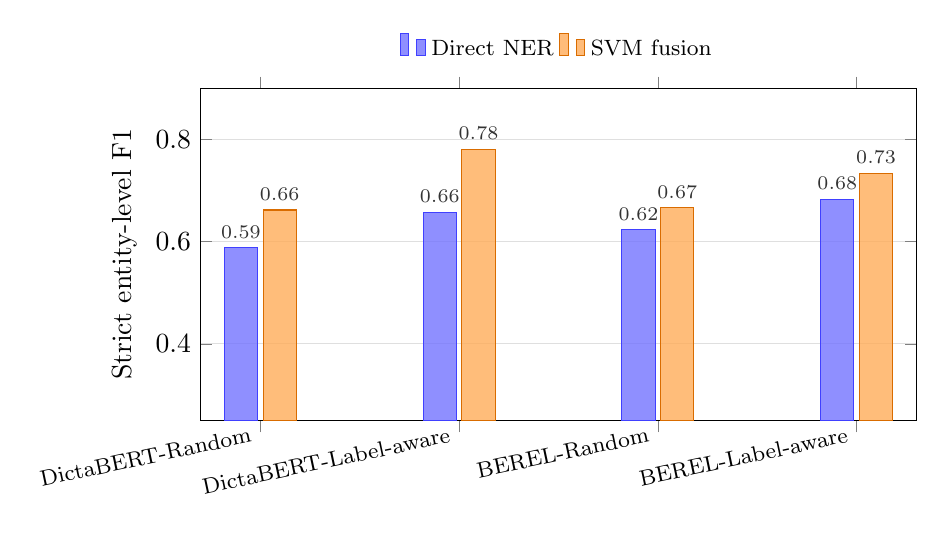
\begin{tikzpicture}
\begin{axis}[
  width=0.88\textwidth,
  height=5.8cm,
  ybar,
  bar width=12pt,
  ymin=0.25,
  ymax=0.90,
  ylabel={Strict entity-level F1},
  symbolic x coords={DictaBERT-Random,DictaBERT-Label-aware,BEREL-Random,BEREL-Label-aware},
  xtick=data,
  x tick label style={font=\footnotesize,rotate=12,anchor=east},
  ymajorgrids=true,
  grid style={gray!25},
  legend style={font=\footnotesize,draw=none,at={(0.5,1.05)},anchor=south,legend columns=2},
  nodes near coords,
  nodes near coords style={font=\scriptsize},
  every axis plot/.append style={fill opacity=0.8,draw opacity=1}
]
\addplot[fill=blue!55,draw=blue!75] coordinates {
  (DictaBERT-Random,0.588) (DictaBERT-Label-aware,0.657) (BEREL-Random,0.623) (BEREL-Label-aware,0.683)
};
\addplot[fill=orange!65,draw=orange!85!black] coordinates {
  (DictaBERT-Random,0.662) (DictaBERT-Label-aware,0.781) (BEREL-Random,0.666) (BEREL-Label-aware,0.734)
};
\legend{Direct NER,SVM fusion}
\end{axis}
\end{tikzpicture}
\caption{Direct-NER and SVM-fusion F1 in one grouped graph for DictaBERT and BEREL 3.0 under random and label-aware splitting.}
\label{fig:results}
\end{figure*}

Figure~\ref{fig:results} visualizes the direct-versus-SVM comparison. SVM fusion improves on direct NER in all four encoder--split conditions; the F1 gains range from 0.042 for BEREL 3.0 under random splitting to 0.124 for DictaBERT under label-aware splitting.

\subsection{Encoder comparison}

BEREL 3.0 outperforms DictaBERT for direct NER under both splits, with F1 values of 0.623--0.683 compared with DictaBERT F1 values of 0.588--0.657. After Holm correction, the paired Wilcoxon tests in Table~\ref{tab:encoder_wilcoxon} show that BEREL's direct-NER advantage is significant at $\alpha=0.01$ for both random and label-aware splitting. SVM fusion reduces dependence on encoder choice: the mean absolute F1 gap between DictaBERT and BEREL across the two splits decreases from 0.031 for direct NER to 0.025 after fusion, a descriptive reduction of approximately 18\%. The reduction is especially clear under random splitting, where the F1 gap decreases from 0.035 to 0.004. DictaBERT is significantly better after fusion under label-aware splitting ($p_H=0.00145$), whereas the small BEREL advantage under random splitting ($p_H=0.898$) is not significant at $\alpha=0.01$.

\begin{table}[!t]
\centering
\caption{Two-sided paired Wilcoxon tests comparing DictaBERT with BEREL 3.0. $\Delta$F1 is DictaBERT minus BEREL; $p_H$ is Holm-adjusted across four tests.}
\label{tab:encoder_wilcoxon}
\scriptsize
\begin{tabular}{@{}llrlrc@{}}
\toprule
Method & Split & $\Delta$F1 & Better & $p_H$ & Sig. .01 \\
\midrule
Direct NER & Random & $-0.035$ & BEREL & $1.45\!\times\!10^{-3}$ & Yes \\
Direct NER & Label-aware & $-0.026$ & BEREL & $3.10\!\times\!10^{-5}$ & Yes \\
SVM fusion & Random & $-0.004$ & BEREL & $0.898$ & No \\
SVM fusion & Label-aware & $\mathbf{+0.046}$ & \textbf{DictaBERT} & $1.45\!\times\!10^{-3}$ & Yes \\
\bottomrule
\end{tabular}
\end{table}

\subsection{Effect of splitting}

Label-aware splitting yields higher direct and SVM-fusion F1 values than random splitting for both encoders. Relative to random splitting, the direct-NER F1 increases by 0.069 for DictaBERT and by 0.060 for BEREL 3.0. These differences demonstrate substantial partition sensitivity in the 150-sentence setting.

\subsection{Effect of the prediction pipeline}

The standalone cascade obtains lower F1 than direct NER, particularly with BEREL 3.0, and deterministic repair has negligible effect on F1. Nevertheless, it provides predictions that complement the direct model. Confidence fusion does not exploit this complementarity consistently, whereas the learned router produces the highest F1 for both encoders under every split.

\subsection{Baseline significance tests}

All four SVM-fusion configurations significantly outperform the encoder-specific Random-split Direct-NER baseline after Holm correction at $\alpha=0.01$ (Table~\ref{tab:wilcoxon}). The F1 gains range from $+0.042$ for BEREL 3.0 with random splitting to $+0.193$ for DictaBERT with label-aware splitting.

\begin{table}[!t]
\centering
\caption{Two-sided paired Wilcoxon tests against the encoder-matched Random Direct-NER baseline. $p_H$ is Holm-adjusted across four tests.}
\label{tab:wilcoxon}
\scriptsize
\begin{tabular}{@{}llrrc@{}}
\toprule
Encoder & SVM split & $\Delta$F1 & $p_H$ & Sig. at .01 \\
\midrule
BEREL 3.0 & Random & +0.042 & $7.63\!\times\!10^{-5}$ & Yes \\
BEREL 3.0 & Label-aware & +0.111 & $2.65\!\times\!10^{-4}$ & Yes \\
DictaBERT & Random & +0.073 & $2.65\!\times\!10^{-4}$ & Yes \\
DictaBERT & Label-aware & $\mathbf{+0.193}$ & $2.65\!\times\!10^{-4}$ & \textbf{Yes} \\
\bottomrule
\end{tabular}
\end{table}

\section{Discussion}

BEREL 3.0 achieves significantly higher direct-NER F1 than DictaBERT under both splits, supporting domain-matched pretraining. After SVM fusion, the average absolute F1 gap between the encoders is reduced, indicating that learned routing makes F1 less sensitive to encoder selection. The highest overall F1 is obtained with DictaBERT, but its fused F1 advantage is significant only with label-aware splitting. Standalone encoder quality and complementarity between direct and decomposed predictions are therefore distinct properties.

Partition composition is a substantive source of variance. Label-aware splitting produces higher direct and fused F1 values than random splitting for both encoders, showing that controlled label allocation is more informative than relying on one random estimate.

The cascade is useful as a complementary source rather than a replacement for direct NER. Its standalone F1 is lower, but its distinct predictions provide disagreements that the SVM router exploits more effectively than confidence fusion.

\subsection{Limitations}

The SVM-fusion results are exploratory because the router was learned from labeled disagreements in the available prediction set. A stricter protocol should use out-of-fold predictions or a dedicated development partition and reserve an untouched final test set.

External validity is limited by the 150-sentence sample and the scarcity of several labels; section prefixes, for example, account for only 10 entity tokens. The reported Wilcoxon tests quantify consistency across the recorded seed-aligned runs, not generalization to additional Responsa collections. Larger corpora are required for reliable per-class and multi-token-span analysis.

\section{Conclusion}

We evaluated fine-grained reference-component extraction from 150 Hebrew-Aramaic Responsa sentences. BEREL 3.0 was the stronger direct recognizer, while DictaBERT with label-aware splitting and SVM routing achieved the highest strict entity-level F1 of 0.781. Future work should validate routing out of fold on a larger annotated corpus with an untouched test set.

\begin{thebibliography}{99}
\sloppy

\bibitem{hacohen2010}
Y. HaCohen-Kerner, M. Zohar, and D. Mughaz,
``Automatic identification of biblical quotations in Hebrew-Aramaic documents,''
\emph{Cybernetics and Systems}, vol. 41, no. 3, pp. 180--197, 2010.

\bibitem{hacohen2010haads}
Y. HaCohen-Kerner, A. Kass, and A. Peretz,
``HAADS: A Hebrew Aramaic abbreviation disambiguation system,''
\emph{Journal of the American Society for Information Science and Technology}, vol. 61, no. 9, pp. 1923--1932, 2010.

\bibitem{mordecai2005hebrew}
N. B. Mordecai and M. Elhadad,
``Hebrew named entity recognition,''
\emph{MONEY}, vol. 81, pp. 82--49, 2005.

\bibitem{itai2008}
A. Itai and S. Wintner,
``Language resources for Hebrew,''
\emph{Language Resources and Evaluation}, vol. 42, pp. 75--98, 2008.

\bibitem{tsarfaty2019hebrewnlp}
R. Tsarfaty, S. Sadde, S. Klein, and A. Seker,
``What's wrong with Hebrew NLP? and how to make it right,''
in \emph{Proc. EMNLP-IJCNLP System Demonstrations}, pp. 259--264, 2019.

\bibitem{lafferty2001crf}
J. Lafferty, A. McCallum, and F. Pereira,
``Conditional random fields: Probabilistic models for segmenting and labeling sequence data,''
in \emph{Proc. ICML}, pp. 282--289, 2001.

\bibitem{ma2016bilstmcrf}
X. Ma and E. Hovy,
``End-to-end sequence labeling via bidirectional LSTM-CNNs-CRF,''
in \emph{Proc. ACL}, pp. 1064--1074, 2016.

\bibitem{devlin2018bert}
J. Devlin, M.-W. Chang, K. Lee, and K. Toutanova,
``BERT: Pre-training of deep bidirectional transformers for language understanding,''
\emph{arXiv:1810.04805}, 2018.

\bibitem{li2022ner}
J. Li, A. Sun, J. Han, and C. Li,
``A survey on deep learning for named entity recognition,''
\emph{IEEE Transactions on Knowledge and Data Engineering}, vol. 34, no. 1, pp. 50--70, 2022.

\bibitem{shmidman2023dictabert}
A. Shmidman, S. Shmidman, and M. Koppel,
``DictaBERT: A state-of-the-art BERT suite for Modern Hebrew,''
\emph{arXiv:2308.16687}, 2023.

\bibitem{shmidman2022berel}
A. Shmidman, J. Guedalia, S. Shmidman, C. S. Shmidman, E. Handel, and M. Koppel,
``BEREL: BERT embeddings for rabbinic-encoded language,''
in \emph{Proc. Workshop on Language Technologies for Historical and Ancient Languages}, pp. 49--54, 2022.

\bibitem{nguyen2023auc}
N. D. Nguyen, W. Tan, L. Du, W. Buntine, R. Beare, and C. Chen,
``AUC maximization for low-resource named entity recognition,''
in \emph{Proc. AAAI}, vol. 37, no. 11, pp. 13389--13399, 2023.

\bibitem{japkowicz2002}
N. Japkowicz and S. Stephen,
``The class imbalance problem: A systematic study,''
\emph{Intelligent Data Analysis}, vol. 6, no. 5, pp. 429--449, 2002.

\bibitem{kohavi1995}
R. Kohavi,
``A study of cross-validation and bootstrap for accuracy estimation and model selection,''
in \emph{Proc. IJCAI}, pp. 1137--1143, 1995.

\bibitem{sokolova2009measures}
M. Sokolova and G. Lapalme,
``A systematic analysis of performance measures for classification tasks,''
\emph{Information Processing \& Management}, vol. 45, no. 4, pp. 427--437, 2009.

\end{thebibliography}

\end{document}